\begin{frame}{Architettura}
    \begin{figure}[!hb]
        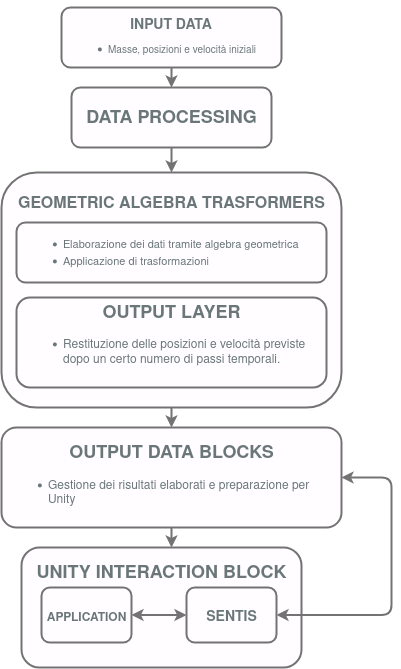
\includegraphics[scale = .325]{../Images/Architecture.png}
    \end{figure}
\end{frame}

\begin{frame}
    La precedente architettura mostra come simulare e visualizzare l'N-body problem combinando una rete neurale basata su Geometric Algebra Transformer e Unity Sentis.
    Nel dettaglio l'architettura è composta dai seguenti moduli principali:
    \begin{enumerate}
        \item Input Data: riceve i parametri fondamentali per rappresentare il problema
        \item Data Preprocessing: i dati grezzi vengono normalizzati e codificati in algebra geometrica proiettiva 
        \item Geometric Algebra Transformer: modella in modo efficiente le interazioni gravitazionali tra i corpi in moto e gli outliers vengono rimossi
        \item Output Data Block: i dati generati dal modello vengono gestiti per permettere una corretta comunicazione con Unity
        \item Unity Interaction Block: stabilisce la comunicazione bidirezionale tra la rete neurale e l'applicazione Unity
    \end{enumerate}
\end{frame}

\begin{frame}{Input Data}
    Questo modulo riceve in input:
    \begin{itemize}
        \item le masse dei pianeti
        \item le coordinate spaziali dei pianeti all'inizio della simulazione
        \item le velocità iniziali descritte da vettori che ne indicano direzione e modulo, fornite dalla velocità di un'orbita circolare stabile.
    \end{itemize}
    Le posizioni iniziali dei pianeti vengono campionate su un cerchio bidimensionale attorno all'origine sul piano x-y, mentre la stella è posizionata in (0, 0) e inizialmente a riposo.
    
\end{frame}

\begin{frame}{Data Preprocessing}
    I dati in input vengono rappresentati secondo due tipi principali di rappresentazione:
    \begin{itemize}
        \item multivettori basati sull'algebra geometrica proiettiva G(3,0,1)
        \item rappresentazioni scalari ausiliarie, che forniscono informazioni supplementari ai multivettori
    \end{itemize}
    I multivettori vengono quindi rappresentati tramite tensori a 16 componenti mentre  le rappresentazioni scalari non hanno una struttura fissa
     ma devono comunque corrispondere nelle dimensioni di batch e numero di elementi ai multivettori a cui sono associate
\end{frame}

\begin{frame}{Geometric Algebra Transformer}
    Questo modulo si occupa di applicare trasformazioni casuali e permutazioni alle posizioni fornite, in modo da generare configurazioni casuali del sistema.
    La posizione e velocità finale dei pianeti vengono calcolate applicando l'equazioni del moto di Newton, i campioni la cui distanza tra la posizione iniziale e finale supera un limite vengono considerati outliers e rimossi.
    Quindi il modulo restituisce la configurazione dei pianeti dopo l'evoluzione temporale e la traiettoria: un array 4D contenente le posizioni di tutti gli oggetti per ogni passo temporale.
\end{frame}{}

\begin{frame}{Output Data Block}
    In questa fase le posizioni ad ogni istante temporale, codificate tramite multivettori, vengono trasformate in punti grezzi per consentire l'interfacciamento con Unity. Inoltre la rete crea un file ONNX che verrà importato in Sentis e permetterà la comunicazione tra l'applicazione e la rete neurale
\end{frame}

\begin{frame}{Unity Interaction Block}
    I dati forniti dall'Output Data Block vengono utilizzati per fornire una rappresentazione 3D e interattiva dell'N-Body problem in cui l'utente può scegliere la posizione iniziale, massa e velocità dei pianeti e della stella e osservare la simulazione tramite visore 
\end{frame}
